%\exer{Implémentation des graphes par une matrice d'adjacence d'un graphe pondéré}


\section*{Snakes and Ladders - Partie 2}

La première partie a déjà été traitée et elle porte sur l'algorithme glouton et les dictionnaires. Le sujet et la correction sont disponibles sur le site de la classe.

\subsection*{Présentation du jeu}

Le jeu \emph{serpents et échelles} est un jeu de société où on espère monter les échelles en évitant de trébucher sur les serpents. Il provient d'Inde et est utilisé pour illustrer l'influence des vices et des vertus sur une vie.

\begin{figure}[h]
	\begin{center}
		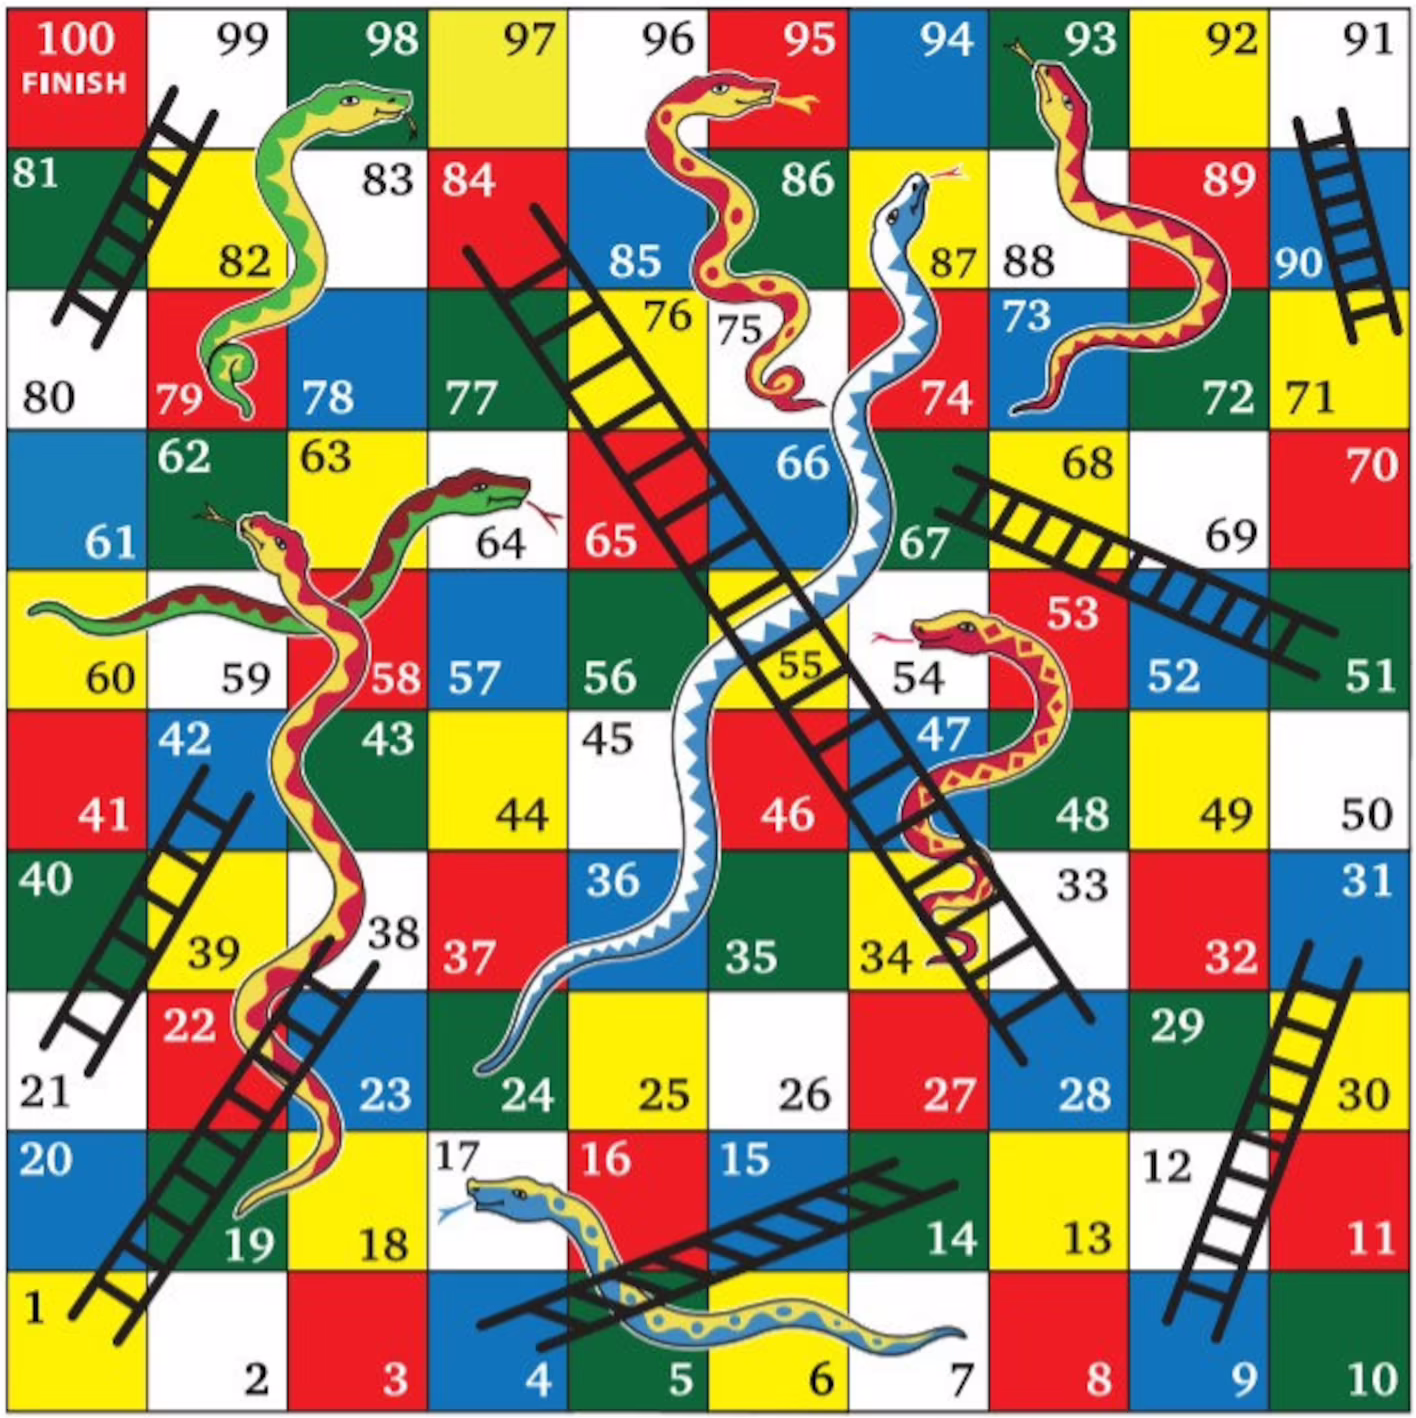
\includegraphics[width=0.6\linewidth]{snakesAndLadders.png}
	\end{center}
	\caption{Exemple d'un plateau de serpents et échelles}
	\label{fig:1}
\end{figure}

\paragraph*{Le plateau}

\begin{itemize}
	\item Le plateau comporte 100 cases numérotées de 1 à 100 en boustrophédon\footnote{à la manière du bœuf traçant des sillons, avec alternance gauche-droite et droite-gauche}~: le 1 est en bas à gauche et le 100 est en haut à gauche~;
	\item des serpents et échelles sont présents sur le plateau~: les serpents font descendre un joueur de sa tête à sa queue, les échelles font monter un joueur du bas de l'échelle vers le haut.
\end{itemize}

\subsection*{Déroulement}

\begin{itemize}
	\item Chaque joueur a un pion sur le plateau. Plusieurs pions peuvent être sur une même case. Les joueurs lancent un dé à tour de rôle et ils avancent du nombre de cases marqués sur le dé. S'ils atterrissent sur un bas d'échelle ou une tête de serpent, ils vont directement à l'autre bout~;
	\item les joueurs commencent sur une case 0 hors du plateau~: la première case où mettre leur pion correspond donc au premier lancer de dé~;
	\item le premier joueur à arriver sur la case 100 a gagné~; 
	\item il existe 3 variantes quand la somme de la case actuelle et du dé dépasse 100~:
	\begin{itemize}
		\item le rebond~: on recule d'autant de cases qu'on dépasse~;
		\item l'immobilisme~: on n'avance pas du tout si on dépasse~: 
		\item la fin rapide~: on va à la case 100 quoi qu'il arrive. 
	\end{itemize}
\end{itemize}

On utilisera les notations suivantes pour les complexités~: $N_{cases}$, le nombre de cases du plateau (100), et $N_{SeE}$ la somme du nombre de serpents et du nombre d'échelle (16 dans notre exemple). Ces variables ne sont pas déclarées dans le script.

\subsection*{Étude du graphe correspondant}

\begin{figure}[h]
	\begin{center}
		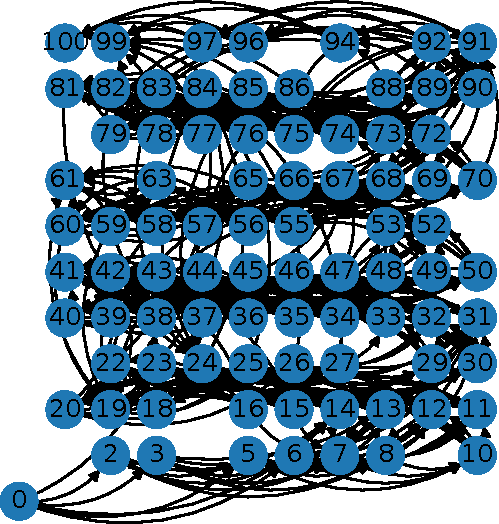
\includegraphics[width=0.4\linewidth]{Graphe}
	\end{center}
	\caption{Graphe correspondant au plateau de la figure 4}
	\label{fig:3}
\end{figure}


\subsection*{Élimination des doublons}

\question{\'Ecrire une fonction \texttt{eliminationDoublon\_naif(L: [int]) -> [int]:} qui renvoie une liste ayant exactement les mêmes éléments, mais sans répétition. Vous n'utiliserez ni dictionnaire, ni tri.}

%\UPSTIcorrection{
%	\lstinputlisting[firstline=39, lastline=44]{trouverCheminPlusCourt.py}
%}


\question{Prouver que cette fonction est de complexité quadratique en la longueur de la liste dans le pire des cas.}

%\UPSTIcorrection{
%	Le pire des cas est quand on n'a aucun doublon~: on a alors un test qui parcourt 0 éléments, puis 1, puis 2, jusqu'à \texttt{len(L) - 1}. Cette somme donne un nombre de comparaisons de $\dfrac{N(N-1)}{2}$ avec $N=$\texttt{len(L)}. 
%	
%	On a donc une complexité en $O(len(L)^2)$. 
%}

\question{\'Ecrire une fonction \texttt{eliminationDoublon\_tri(L: [int]) -> [int]:} ayant une complexité en \newline
$O\left(len(L) \log (len(L)) \right)$ en utilisant un tri sur \texttt{L}.}


\question{Proposer une fonction \texttt{eliminationDoublon\_dict(L: [int]) -> [int]:} ayant une complexité linéaire en la longueur de la liste. Vous pourrez vous aider d'un dictionnaire.}

%\UPSTIcorrection{
%	\lstinputlisting[firstline=46, lastline=53]{trouverCheminPlusCourt.py}
%}

\subsection*{Construction d'un graphe}

On souhaite créer un graphe à partir du jeu~: chaque case stable est un sommet et il existe un arc de la case \texttt{case1} à la case \texttt{case2} si un lancer de dé permet d'aller de \texttt{case1} à \texttt{case2}. On notera que la case \texttt{100} n'a pas de successeurs (puisque le jeu s'arrête). De plus, une case \texttt{0} sera utilisée pour prendre en compte le départ. Une représentation de ce graphe est donnée sur la figure 5.

\question{En vous aidant des fonctions \texttt{casesAccessibles()} et \texttt{eliminationDoublon\_dict()}, construire un graphe orienté \texttt{G} sous la forme d'un dictionnaire d'adjacence (dictionnaire de listes).}

%\UPSTIcorrection{
%	\lstinputlisting[firstline=92, lastline=96]{trouverCheminPlusCourt.py}
%}

\question{Pourquoi a-t-on besoin d'éliminer des doublons~? Prenez un exemple pour illustrer.}

%\UPSTIcorrection{
%Avec la méthode d'immobilisme pour la fin, plusieurs résultats de dé ont le même effet~: or, on ne souhaite pas qu'un même arc apparaisse plusieurs fois dans le dictionnaire d'adjacence. 
%}

\question{Quel est le nombre de sommets de ce graphe en fonction de $N_{cases}$ et $N_{seE}$.}

%\UPSTIcorrection{
%	$N_{cases} - N_{seE} + 1$~: on a autant de cases non stables que de serpents et d'échelles, mais il faut ajouter la case 0. 
%}

Afin de résoudre le problème du parcours à nombre de coups minimum, on a mis au point une fonction qui trouve si un chemin existe entre un sommet de départ et un sommet d'arrivée~: 

\noindent \lstinputlisting[firstline=55,lastline=65]{trouverCheminPlusCourt.py}

\question{Sur quel type de parcours est basée la fonction \texttt{chemin}~? Justifiez cette réponse. Précisez l'intérêt d'utiliser ce parcours ?}

%\UPSTIcorrection{
%	Les frères sont recherchés avant les fils, on utilise une file~: on a donc un parcours en largeur. 
%}

Pour l'instant, la fonction renvoie un booléen, mais on souhaiterait qu'elle renvoie l'ensemble des cases par lesquelles on est passé pour passer de \texttt{depart} à \texttt{arrivee} avec, comme premier élément de la liste retournée \texttt{depart} et comme dernier élément de la liste retournée \texttt{arrivee}. La fonction renverra une liste vide si aucun chemin n'a été trouvé. 

\question{Remplacer la ligne 11 par un ensemble de lignes permettant de répondre à cette exigence.}

%\UPSTIcorrection{
%	\lstinputlisting[firstline=67, lastline=87]{trouverCheminPlusCourt.py}
%}

\question{\'Ecrire une fonction \texttt{partieOptimale() -> [int]} qui renvoie une liste de case à longueur minimum partant de 0 et arrivant à 100 en vous aidant de la fonction mise en place précédemment.}

%\UPSTIcorrection{
%	\lstinputlisting[firstline=89, lastline=90]{trouverCheminPlusCourt.py}
%}

Cette dernière fonction nous renvoie \texttt{[0, 38, 39, 45, 67, 91, 94, 100]}. Pour ce plateau, elle ne nous donne pas une partie plus courte que l'algorithme glouton, et un chemin qui n'est pas fondamentalement différent.

\subsection*{Dessiner le plateau}

On souhaite faire une représentation schématique du plateau (voir figure 6) avec le code suivant~: 

\noindent\lstinputlisting[firstline=13,lastline=29]{dessinerPlateau.py}

\begin{figure}[h]
	\begin{center}
		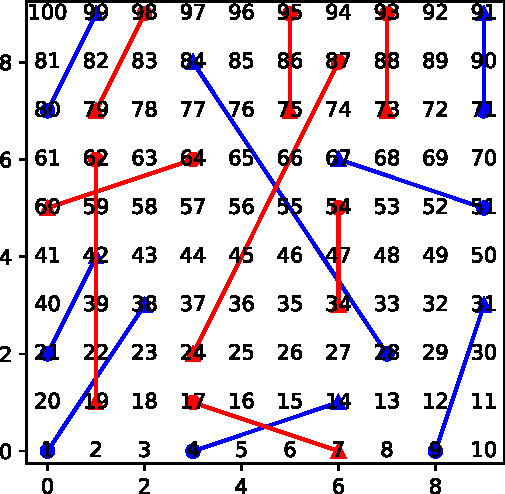
\includegraphics[width=0.4\linewidth]{Plateau}
	\end{center}
	\caption{Représentation schématisée du plateau de la figure 4}
	\label{fig:2}
\end{figure}

\question{\'Ecrire une fonction \texttt{position(case: int) -> (int, int)} qui renvoie les coordonnées de la case numérotée \texttt{case} sous las forme d'un couple d'entier. On doit avoir \texttt{position(1)} qui renvoie \texttt{(0, 0)} (coin en base à gauche) et \texttt{position(91)} qui renvoie \texttt{(9, 9)} (coin en haut à droite).}

%\UPSTIcorrection{
%	\lstinputlisting[firstline=3, lastline=8]{dessinerPlateau.py}
%}

\question{En commentant la ligne 6, dites à quoi correspondent les variables \texttt{caseD} et \texttt{caseA} par rapport au dictionnaire \texttt{dSeE}.}

%\UPSTIcorrection{
%	\texttt{caseD} correspond à une clé et \texttt{caseA} est la valeur correspond à cette clé. \texttt{for caseD, caseA in dSeE.items():} permet donc de parcourir tous les couples (clé, valeur) du dictionnaire \texttt{dSeE}. 
%}

\question{Commenter le rôle des lignes 9 à 12 du code fourni.}

%\UPSTIcorrection{
%	On dessine les échelles en bleu et les serpents en rouge. 
%}




\section*{Annexe}

\subsection*{Utilisation du module \texttt{random}}

On vous donne les docstrings correspondant à deux fonctions du module \texttt{random}~: 

\begin{lstlisting}
randint(a, b) method of random.Random instance
    Return random integer in range [a, b], including both end points.
	
choice(seq) method of random.Random instance
    Choose a random element from a non-empty sequence.
\end{lstlisting}

\subsection*{Complexité des opérations sur les listes et dictionnaires}

\paragraph*{Principales opérations sur les listes}

\texttt{n}, longueur de la liste \texttt{L}, \texttt{k}, un indice valide en négatif (\texttt{1} à \texttt{n}).

\begin{longtable}{|m{9cm}|m{2.1cm}|} \hline
	\bf \centering Opération & \bf \centering Moyen \tabularnewline
	\hline
	\endhead
	Longueur (\texttt{len(L)}) &  $O(1)$ \tabularnewline
	\hline
	Accès en lecture d'un élément &  $O(1)$ \tabularnewline
	\hline
	Accès en écriture d'un élément &  $O(1)$ \tabularnewline
	\hline
	Copie (\texttt{L.copy()} ou \texttt{L[:]}) & $O(n)$ \tabularnewline
	\hline
	Ajout (\texttt{L.append(elt)} ou \texttt{L+=[elt]}) & $O(1)$ \tabularnewline
	\hline
	Extension (\texttt{L1.extend(L2)} ou \texttt{L1+=L2}) & $O(n_2)$ \tabularnewline
	\hline
	Concaténation (\texttt{L1 + L2}) &  $O(n_1 + n_2)$ \tabularnewline
	\hline
	Test de présence (\texttt{elt in L}) & $O(n)$ \tabularnewline
	\hline
	Désempiler dernier (\texttt{L.pop()}) &  $O(1)$ \tabularnewline
	\hline
	Désempiler autre (\texttt{L.pop(-k)}) &  $O(k)$ \tabularnewline
	\hline
	Maximum ou minimum (\texttt{max(L)} et \texttt{min(L)}) &  $O(n)$ \tabularnewline
	\hline
	Tri (\texttt{L.sort()} ou \texttt{sorted(L)}) &  $O(n \log(n))$ \tabularnewline
	\hline
\end{longtable}

\paragraph*{Principales opérations sur les dictionnaires}

\texttt{n}, longueur du dictionnaire \texttt{d}, \texttt{k}, une clé du dictionnaire.

\begin{longtable}{|m{9cm}|m{2.1cm}|} \hline
	\bf \centering Opération & \bf \centering Moyen \tabularnewline
	\hline
	\endhead
	Longueur (\texttt{len(d)}) &  $O(1)$ \tabularnewline
	\hline
	Accès en lecture d'un élément (\texttt{x = d[k]})  &  $O(1)$ \tabularnewline
	\hline
	Accès en écriture d'un élément (\texttt{d[k] = x}) &  $O(1)$ \tabularnewline
	\hline
	Copie (\texttt{d.copy()}) & $O(n)$ \tabularnewline
	\hline
	Ajout (\texttt{d[k] = x} la première fois) & $O(1)$ \tabularnewline
	\hline
	Test de présence (\texttt{k in d}) & $O(1)$ \tabularnewline
	\hline
	Retrait d'un élément (\texttt{del d[k]} ou \texttt{d.pop(k)}) & $O(1)$ \tabularnewline
	\hline
\end{longtable}

\subsection*{Utilisation du module \texttt{matplotlib}}

\texttt{plt.text(x, y, s)} permet de placer la chaine de caractères \texttt{s} aux coordonnées \texttt{(x, y)}. Des arguments optionnels permettent la méthode de placement horizontal (\texttt{horizontalalignment} qui peut prendre les valeurs \texttt{'center'}, \texttt{'right'} ou \texttt{'left'}) et vertical (\texttt{verticalalignment} qui peut prendre les valeurs \texttt{'center'}, \texttt{'top'}, \texttt{'bottom'}, \texttt{'baseline'}, \texttt{'center\_baseline'}).

\texttt{plt.plot(x, y, '\textasciicircum')} permet de placer un point aux coordonnées \texttt{(x, y)} sous la forme d'un triangle vers le haut. Beaucoup d'autres existent, en plus du triangle vers le haut, dont (liste non-exhaustive)~: \texttt{'v'}, \texttt{'<'} et \texttt{'>'} pour des triangles orientés différemment~; \texttt{'.'} et \texttt{'o'} pour des disques plus ou moins gros~; \texttt{'s'}, \texttt{'p'} et \texttt{'h'} pour des figures régulières à 4, 5 ou 6 côtés. 

\texttt{plt.plot(Sx, Sy)} permet de tracer une courbe en trait plein en reliant les points dans l'ordre des 2 séquences données en entrées (le point de coordonnées \texttt{(Sx[i], Sy[i])} est lié au point de coordonnées \texttt{(Sx[i+1], Sy[i+1])}.

Un argument de couleur peut être utilisé avec \texttt{plt.plot}~: des raccourcis existent pour les couleurs le plus fréquentes~: \texttt{'b'} pour bleu, \texttt{'r'} pour rouge, \texttt{'g'} pour vert, \texttt{'c'} pour cyan, \texttt{'m'} pour magenta, \texttt{'y'} pour jaune, \texttt{'k'} pour noir et \texttt{'w'} pour blanc. 

\texttt{plt.axis('equal')} permet de contraindre un ratio de 1 entre l'échelle en abscisses et en ordonnées (repère orthonormé).

\texttt{plt.show()} crée la figure en cours dans une nouvelle fenêtre. 
 







